\graphicspath{{chapters/05/}}
\chapter{Deterministic simulations}

A \emph{deterministic} way of calculating the dynamics of a system, when
the last (noise) term of CLM equation becomes negligibly small compared
with the second one, can be applied. This happens in the limiting case
$*a_j(\mathbf{x})\tau → \inf*$, $*j = 1,...,M*$, and the deterministic
simulation produces an average behaviour of the system that is very
close to the one that results by averaging an infinite number of
stochastic simulations of the system starting from the same initial
state. If we work in terms of \emph{moles}, we are moving Avogrado
numbers; it is not so distant from the reaction size, the assumption is
correct enough. The deterministic simulations should give as an output
the same result as an average stochastic simulation.

ODEs can be safely used to simulate a biochemical system that satisfies
the spatial homogeneity and continuum hypothesis.

\textbf{Continuum hypothesis: ``}A biochemical system satisfies the
continuum hypothesis if the number of molecules for each species is
large enough to safely approximate molecular abundances by
concentrations that vary continuously (as opposed to integer- valued
molecule counts).''

Sometimes, models simply use the ODE formalism, regardless of the
hypothesis (since the ODE is the only computational framework allowing
to reach the end of the simulation).

We are required to apply conversions and derive the ODE according to the
following table:

\begin{figure}
\centering
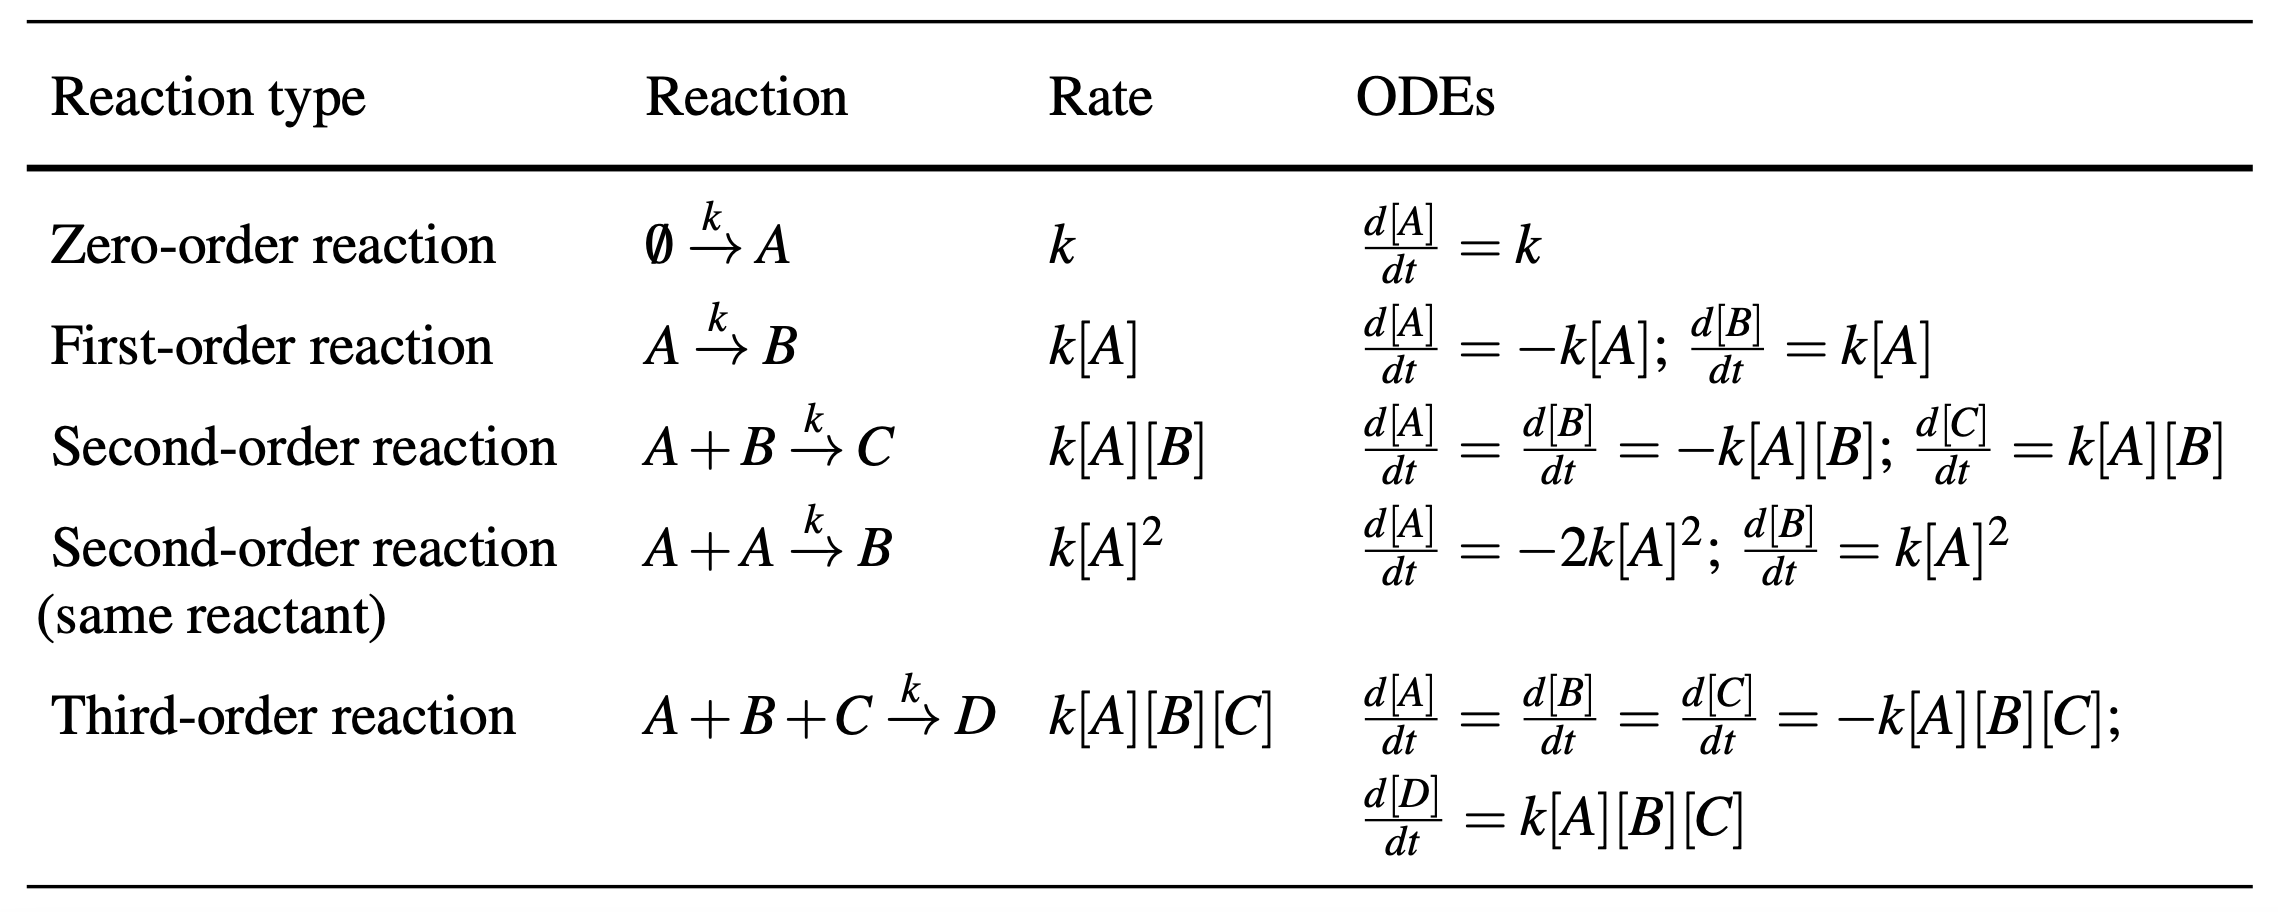
\includegraphics{05_images/reaction_ODEs.png}
\caption{Table 4.4 Marchetti's book}
\end{figure}

Table 4.4 Marchetti's book

Here we are not considering the combination of the reactants. c =
stochastic rate, k = deterministic rate.

\begin{figure}
\centering
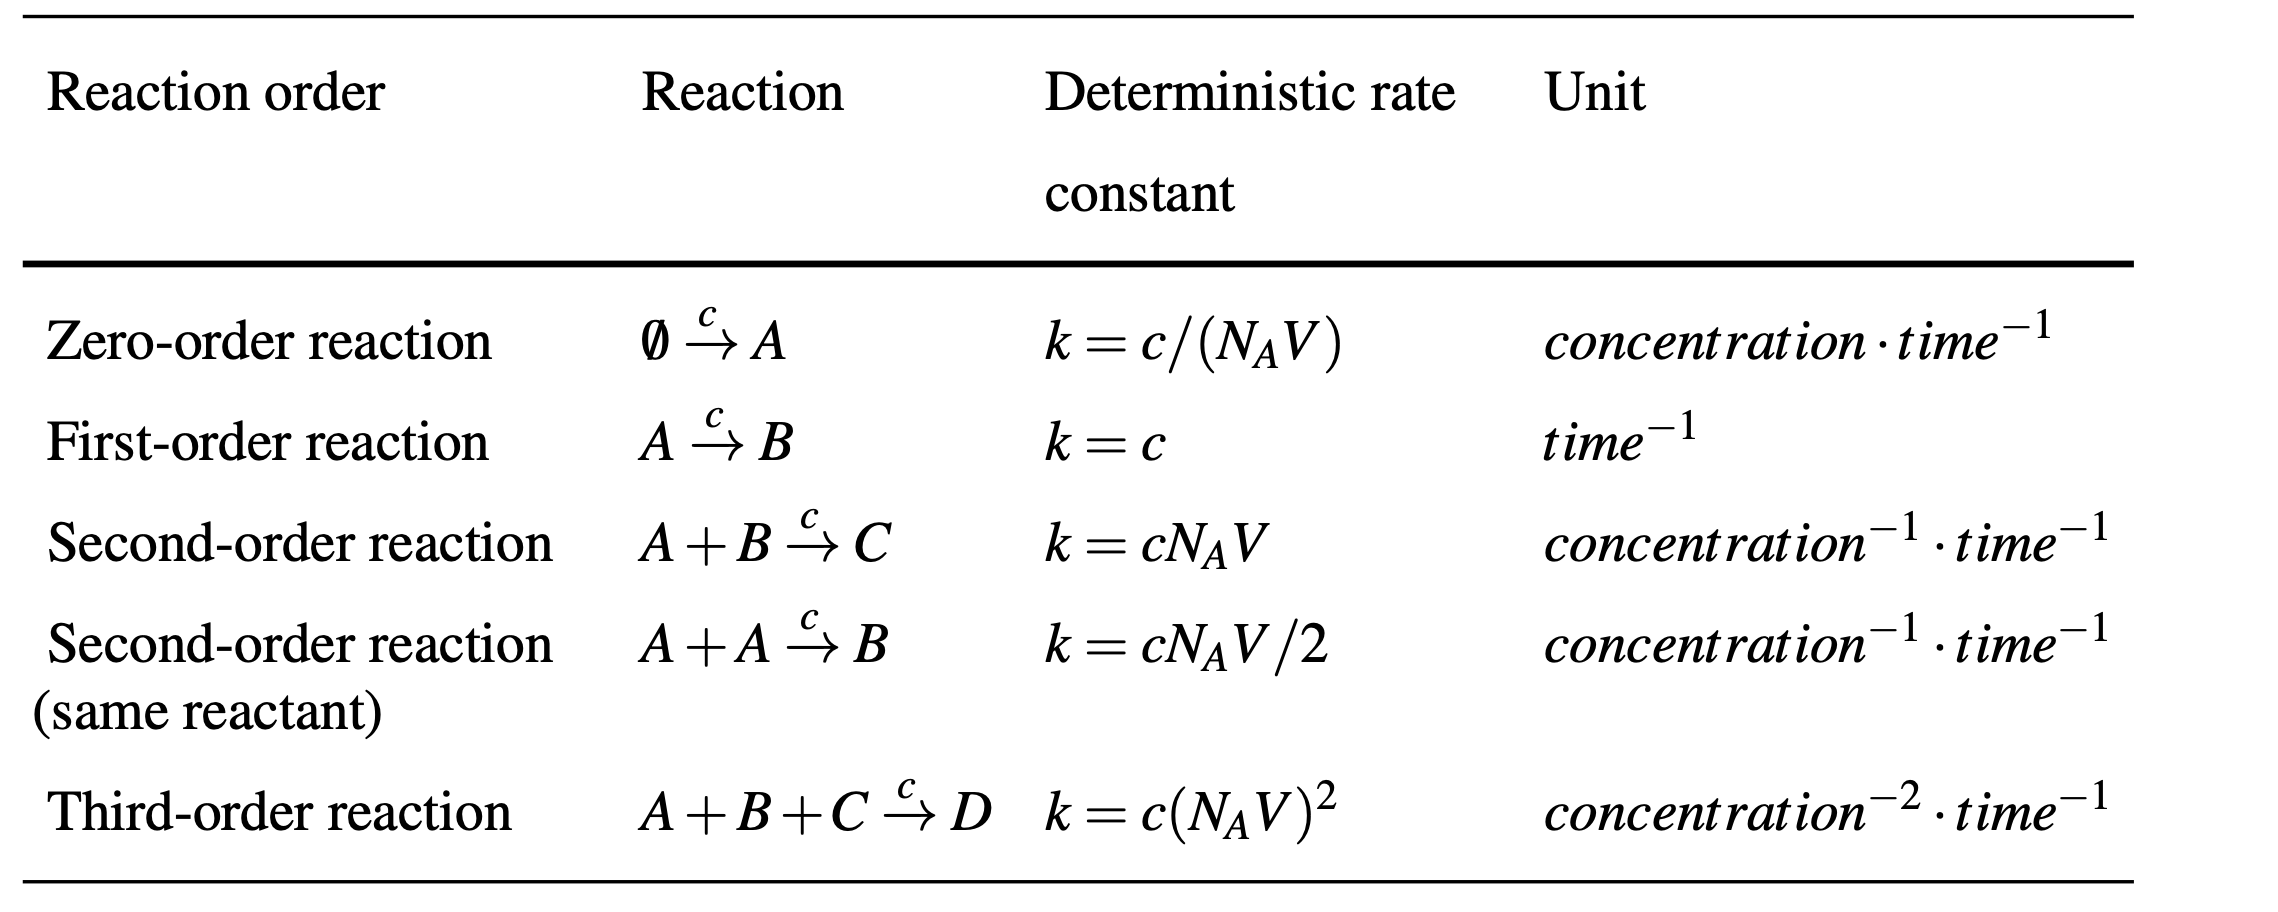
\includegraphics{05_images/reaction_rates.png}
\caption{Table 4.5 Marchetti's book}
\end{figure}

Table 4.5 Marchetti's book

It is possible to go back to the stochastic setting from the
deterministic one.

CLM equation: if we assume that the product is crazily high i.e.~close
to infinite, we can assume that the two parts of the equations have
different orders; in this specific condition, the noise part becomes
negligible.

\hypertarget{deterministic-approximation}{%
\section{Deterministic
approximation}\label{deterministic-approximation}}

If the propensity is approaching infinite, we can assume that the
deterministic setting is motivated. We are required to introduce the law
of mass action and employ tables {[}last lecture{]} to derive a set of
ODEs. In this context, the law of mass action is a bit different from
what we have observed at the beginning of the course. We need to
remember that the constant of proportionality, i.e.~rate, is not the
same as the stochastic setting.

\$\$

\begin{verbatim}
                \\frac{d[S_i]}{dt} = \\sum^M_{j=1}(                  k_j\\mathbf{v}_{ji} \\prod^{N}_{l=1}{[S_l^{\\mathbf{v}^{-}_{jl}}]})            ,i = 1,...,N.
\end{verbatim}

\$\$

The equation $\frac{d[S_i]}{dt}$ should represent a molar concentration
over time. We have an equation for each of the species $i=1,…,N$. It
should take into consideration the effect of all substances in the
system → sum over $M$, considering all reactions, which will be
multiplied by the stoichiometric index. The system is computed as $k$
(constant of proportionality), stoichiometric index and the product of
all the reactants. If a species is not a reactant, $S_i=0$, we end up
with 1, only product of the reactants.

$$
\frac{d[A]}{dt} = - \frac{d[B]}{dt}= -V_{MAX} \cdot \frac{[A]}{K_M+[A]}
$$

We can just rely on a simplified set of equations to avid mass action
correspondence. $V_{MAX}$ = maximum velocity of the enzymatic reactions,
$K_m$, called \emph{Michaelis constant}, indicates the concentration of
the substrate at which the reaction rate is half of its maximum value.

\hypertarget{numerical-solution-of-odes}{%
\section{Numerical solution of ODEs}\label{numerical-solution-of-odes}}

Often times in computational biology it is unlikely to have enough power
for deriving an analytical solution of the system, reality is different
and the complexity prevents this kind of approach. Therefore we rely on
numerical methods to compute the simulation, adding an additional layer
of approximation. The algorithm uses the idea of derivative to
understand the next value. For a value of t\textgreater0, the level of
approximation could be remarkable and depends on the dynamics of the
system.

Remember that when we simulate in time we have the issue that the
computation of the next state depends on the previous state: we are
dealing with an iterative formula, so potentially we can have a huge
error explosion. At the basis of such method is the concept of
derivative and geometrical rule to identify next step; Euler's method is
the simplest one.

\hypertarget{eulers-method}{%
\subsection{Euler's method}\label{eulers-method}}

The first examples of explicit/implicit numerical methods are the
\emph{forward Euler method/backward Euler method} for updating the
system state:

\begin{itemize}
\tightlist
\item
  Forward Euler: $[X_{n+1}] = [X_n]+h·F(t_n,[X_n])$
\item
  Backward Euler: $[X_{n+1}] = [X_n]+h·F(t_{n+1},[X_{n+1}])$
\end{itemize}

Not surprisingly, for increasing the order of the algorithm we will
require a more accurate approx of the derivative, translating in
additional evaluation of the ODE.

\hypertarget{runge-kutta-method}{%
\subsection{RUNGE-KUTTA Method}\label{runge-kutta-method}}

RK4 is a 4th order method, good compromise in accuracy and computational
requirements. This algorithm uses a sort of average over Ks, which are
computed by solving the set of ODEs as following:

$*K1 = F(t_n,[X_n])\\ K2 = F(t_n + 2h,[X_n]+ h2K_1)*$

$*K3 = F(t_n + h2,[X_n]+ h2K_2)\\ K4 = F(t_{n+1},[X_n]+h·K_3)*$

Is it possible to increase accuracy without increasing complexity?

``{[}entra una ragazza in classe, dice ``ups'', esce imbarazzata perché
ha sbagliato aula{]} M: ahaha. SERIO,DETERMINISTICO''

\hypertarget{midpoint-method}{%
\subsection{Midpoint method}\label{midpoint-method}}

2nd order method, we compute the new state at line 5 by two elements: x
the current state and x old (the previous one). In this case, the
multi-step method links the increased order to the number of step
previously considered to compute the slope.

Drawback: what happens in the first step? We require an initial state
and and additional time series!

Limitation of multi-step algorithms: they all require a discretization
step, it rules the movement. The time should not be computed during the
iteration, chosen from the beginning; if we think about this, it can be
a limitation of the application of the methodologies, which ask the user
an information which might be unknown. Which is the right time for
simulating? Of course we can try to keep the discretization step as
small as possible, but the right question that should be asked is: which
is the error value? Keeping the error below a certain threshold is not
easy, since the dynamics evolve with the system. In order to achieve
error control, we should apply more requirements to discretization,
leading us to seek an \emph{adaptive solution}.

In order to derive a rough estimate of the error we should compare the
state computed by two algorithms of different order: one should be more
accurate than the other, to have an idea of the degree of approximation.

\hypertarget{adaptive-methods---runge-kutta-fehlberg}{%
\subsection{Adaptive methods -
Runge-Kutta-Fehlberg}\label{adaptive-methods---runge-kutta-fehlberg}}

``Strapopular algorithm: Runge-Kutta-Fehlberg, RK45 for friends''.

\textbf{RK45:} two methods, 4th and 5th order to apply error evaluation
{[}4th for dynamics, 5th for estimating the error{]}. The algorithm will
scale the step (h), in such a way that we keep the deviation below an
error threshold. A formula will allow to play with h according to the
deviation (increase if deviation is little).

Recall that for the 5th order we require 6 derivations. The two methods
are similar, they share the same Ks, therefore at the price of computing
a fifth order method we will have the possibility to obtain two
evaluations → quite efficient method. ODE45 is this algorithm!

Error computation:
$\Delta_{n+1}=\frac{|[\tilde{X}*{n+1}]-[X*{n+1}]|}{h}$

The error estimate is then compared to the error threshold $\epsilon_t$
provided by the user. If $\Delta_{n+1} \leq \epsilon_t$, the local truncation error is
assumed to be smaller than the threshold, the state $[X_{n+1}]$ is
accepted and the algorithm moves one step forward. In the other case,
the new state is not accepted and the next state is evaluated again
using a different (smaller) value of h. In both cases, the value of h is
updated as

$$
h_{n+1}=h_n\sigma \\ \sigma =(\frac{\epsilon_t}{2\Delta_{n+1}})^{1/4}
$$

Issue: it's possible that for specific dynamics we will need an
infinitesimal h to satisfy the error threshold. We can avoid this by
updating the strategy, for instance impose an additional threshold to h
or insert an heuristic.

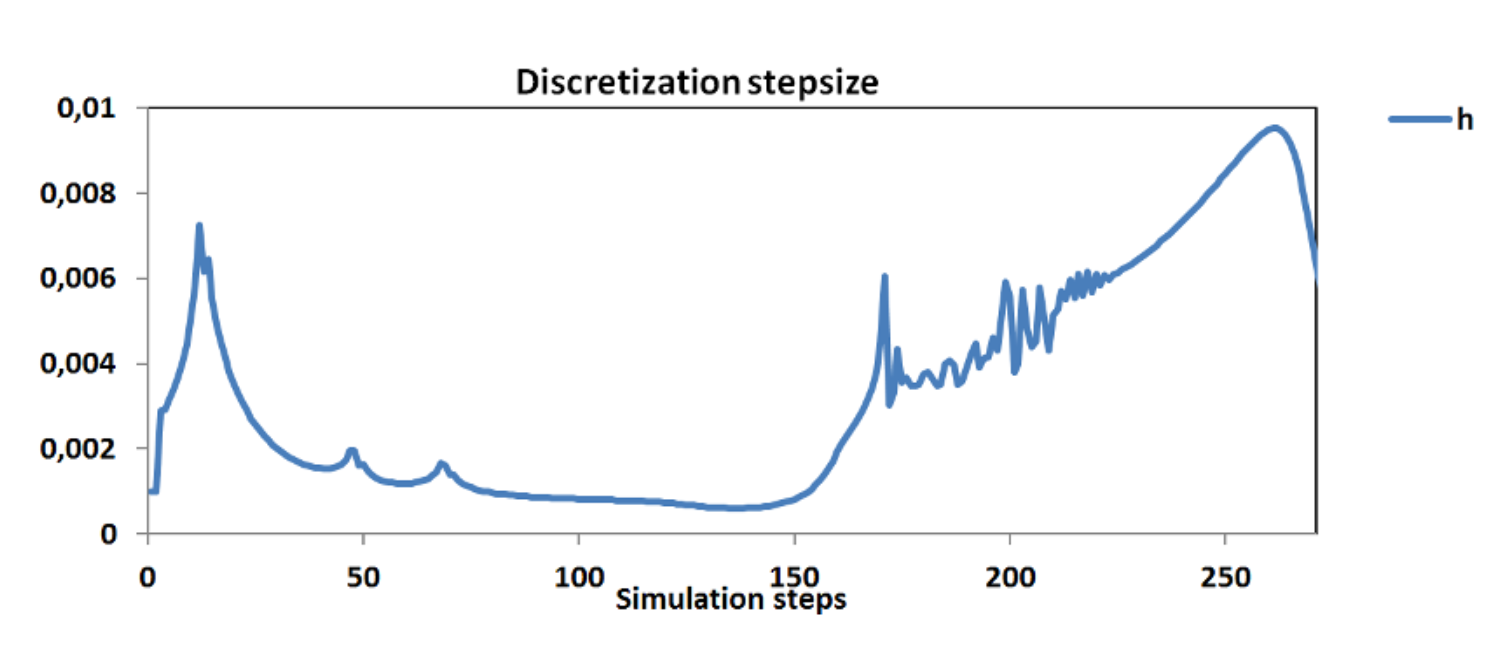
\includegraphics{05_images/discretization.png}

Figure 4.9. Value of h used at each step

We can end up in situations in which the system changes a lot →
\emph{stiffness condition}, if we work with an adaptive method the
property of the dynamics leads to instability in deriving the
discretization step. Stiffness is a couple property of ODEs and the
numerical scheme used to solve the system. This means that the same
system of ODEs may exhibit stiffness only when it is simulated with some
of the numerical schemes introduced in this chapter. In MATLAB we can
use ODE15S in case of stiffness (happens quite often in biology
simulations).
